\documentclass[a4paper,11pt,twoside]{scrartcl}
\usepackage[T1]{fontenc}
\usepackage[utf8]{inputenc}
\usepackage{geometry}
\geometry{left=25mm, right=15mm, bottom=25mm}
\setlength{\parindent}{0em} 
\setlength{\headheight}{0em}
\input{../head/lstlisting.tex}
\usepackage{float}
\usepackage[section]{placeins}
\usepackage{epstopdf}
\usepackage{wrapfig}
\usepackage{caption}
\usepackage{subcaption}
\usepackage{graphicx}
\usepackage{pgfplots}
\usepackage[usenames,dvipsnames,svgnames,table]{xcolor}
\usetikzlibrary{plotmarks}
\usetikzlibrary{patterns}
\usetikzlibrary{decorations.pathmorphing}
\usetikzlibrary{calc}
\usetikzlibrary{shapes}
\begin{document}
	\section{Aufgabe 1: Weighted-Circuit-Satisfiability(WCS) (5+5=10 Punkte)}
	\begin{figure}[H]
		\centering
		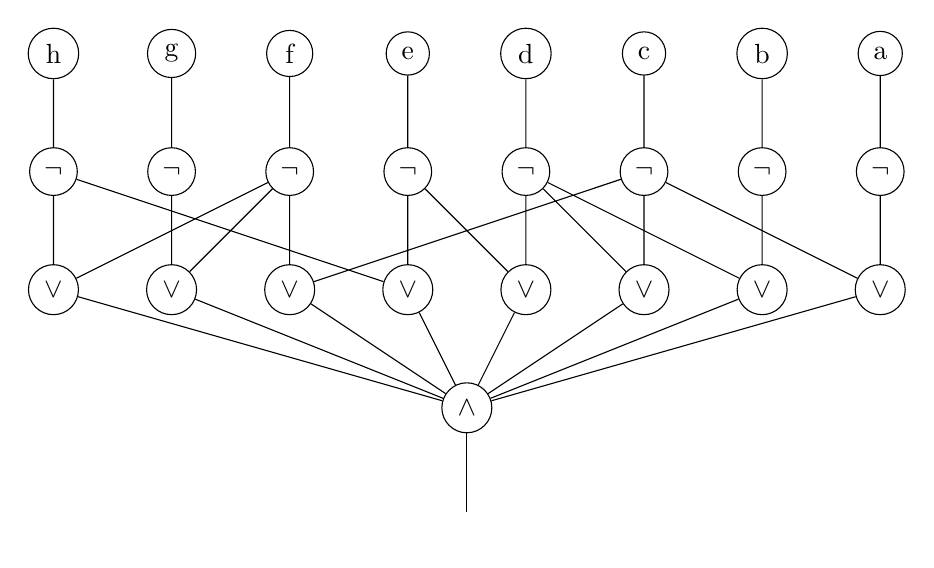
\begin{tikzpicture}[every node/.style = {draw, align=center, circle}, rotate = 180]
		\node[draw = white] {}
		child {
			node {$\land$}
			child {
				node (ac){$\lor$}
				child {
					node (a){$\neg$}
					child {node {a}}	
				}
			}
			child {
				node (bd){$\lor$}
				child {
					node (b){$\neg$}
					child{node {b}}	
				}
			}
			child {
				node (cd) {$\lor$}
				child {
					node (c) {$\neg$}
					child{node{c}}	
				}	
			}
			child {
				node (de) {$\lor$}
				child {
					node(d){$\neg$}
					child{node{d}}
				}	
			}
			child {
				node (eh) {$\lor$}
				child {
					node(e){$\neg$}
					child{node{e}}	
				}	
			}
			child{
				node (cf) {$\lor$}
				child {
					node (f) {$\neg$}
					child{node{f}}	
				}	
			}
			child {
				node (fg) {$\lor$}
				child {
					node(g) {$\neg$}
					child{node{g}}	
				}
			}
			child {
				node (fh) {$\lor$}
				child {
					node(h) {$\neg$}
					child{node{h}}
				}	
			}
		};
		\draw (c) -- (ac) (d)--(bd) (d) -- (cd) (e)--(de) (h)--(eh) (c)--(cf) (f)--(fg) (f)--(fh);
		\end{tikzpicture}
		\caption{a}
	\end{figure}
	\begin{figure}[H]
		\centering
		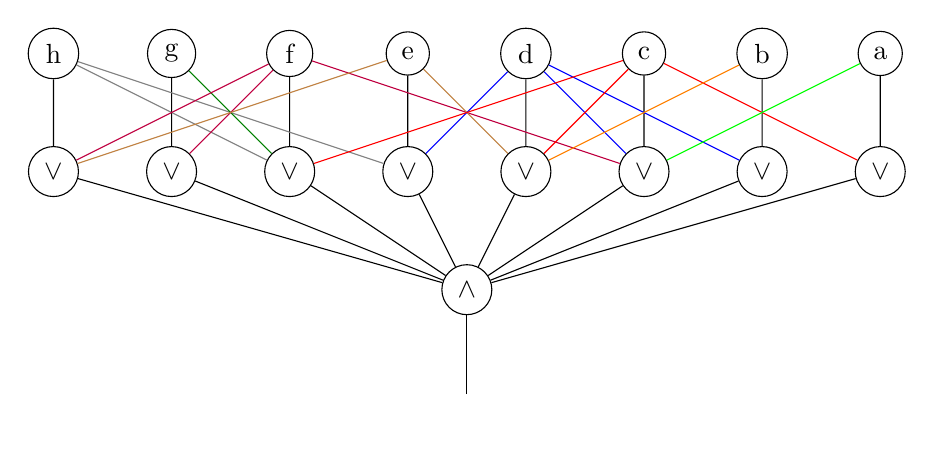
\begin{tikzpicture}[every node/.style = {draw, align=center, circle}, rotate = 180]
		\node[draw = white] {}
		child {
			node {$\land$}
			child {
				node (A) {$\lor$}
				child {
					node (a){a}	
				}
			}
			child {
				node (B){$\lor$}
				child {
					node (b) {b}	
				}
			}
			child {
				node (C){$\lor$}
				child {
					node (c){c}	
				}
			}
			child {
				node (D){$\lor$}
				child {
					node (d){d}	
				}
			}
			child {
				node (E){$\lor$}
				child {
					node (e){e}	
				}
			}
			child {
				node (F){$\lor$}
				child {
					node (f){f}	
				}
			}
			child {
				node (G){$\lor$}
				child {
					node (g){g}	
				}
			}
			child {
				node (H){$\lor$}
				child {
					node (h){h}	
				}
			}
		};
		\draw (c) edge[red] (A) (d) edge[blue] (B) (a) edge[green] (C) (f) edge[purple] (C) (d) edge[blue] (C) (c) edge[red] (D) (e) edge[brown] (D) (b) edge[orange] (D) (d) edge[blue] (E)	(h) edge[gray] (E) (c) edge[red] (F) (h)edge[gray](F) (g)edge[Green](F) (f)edge[purple](G) (f)edge[purple](H) (e)edge[brown](H);
		
		\end{tikzpicture}
		\caption{b}
	\end{figure}
\end{document}